\documentclass[a4paper,10pt]{article}
\usepackage{graphicx}



%opening
\title{Ticket 23: Support for taggin}
\author{Group 3}

\begin{document}

\maketitle

\begin{abstract}

Matthew said RSP uses their naming convention for files, internally.  This is a general ticket on how files should be tagged.  A couple of suggestions is to use key-values pairs as metadata

\end{abstract}

\section{Design}

There will be two tables incorporated to the already existing schema.  This tables are \textit{tag} and \textit{file\_tag}. See figure \ref{fig:TagsTables}

\begin{figure}[h]
 \centering
 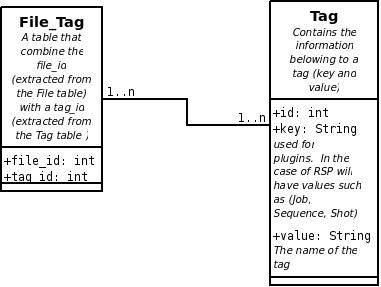
\includegraphics[scale=0.5]{/home/jon/segp2/Subgroups/Group_3/Documents/Designs/ticket23/tag.jpg}
 % tag.jpg: 0x0 pixel, 0dpi, nanxnan cm, bb=
 \caption{Tables to be incorporated into the DB Schema}
 \label{fig:TagsTables}
\end{figure}

This design is done in order to keep the tag as general as possible.  The column \textit{Key} in the \textit{tag} table will change according to the plugin in used.  If no plugin is used, the value of the \textit{Key} will be the same as the Value.  In the case of RSP, the value of the \textit{Key} will be either Job, Sequence or Shot.

The idea is that the plugin used will populate the table given the right \textit{Key}.  And it will also incorporate the ability of seraching according to the \textit{Keys} used


\end{document}
